\chapter{Cinématique}

La cinématique est l'étude du mouvement, sans égard à ce qui cause ce
mouvement.  Nous allons étudier trois catégories principales de mouvements, soit
le mouvement rectiligne uniforme (MRU), le mouvement rectiligne uniformément
accéléré (MRUA), et le mouvement circulaire uniforme (MCU).  Ces catégories se
retrouvent dans un grand nombre d'applications et sont à la base de plusieurs
modèles physiques.


\section{Types de mouvements}

\begin{marginfigure}
  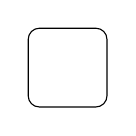
\begin{tikzpicture}[scale=1]
    \draw[rounded corners] (0, 0) rectangle (1, 1);
  \end{tikzpicture}
\end{marginfigure}
Dans ce cours, nous considérerons des mouvements de \textbf{translation},
\textbf{rotation}, et de \textbf{vibration}.  On dit qu'un objet subit une
translation lorsque tous les points qui le composent subissent le même
déplacement.  Une rotation change l'orientation d'un objet dans l'espace.  Une
vibration correspond à un mouvement dans lequel la position des différentes
parties du corps varie périodiquement.

Souvent, lorsque nous considérons un mouvement de translation, on peut
considérer le corps comme une \textbf{particule}.  Une particule peut donc
représenter un objet de dimension considérable (comme une voiture ou une
planète) en autant que la forme exacte de l'objet et sa structure interne
soient sans importance dans le problème que nous considérons.


\section{Caractérisation du mouvement}

Un objet est en mouvement si sa position change au fil du temps.  Il est donc
primordial de bien définir la position, le changement de position (le
déplacement) et la façon dont la position change (vitesse et accélération).

La \textbf{position}, $\vec{r}$, d'un objet est un vecteur qui va de l'origine
du système de coordonnées jusqu'à l'objet lui-même.  En deux dimensions, on
peut écrire
\[
  \vec{r} = x \xhat + y \yhat
\]
Si l'objet a des dimensions considérables par rapport à la situation physique,
définir la position peut être complexe et la ``bonne'' façon de le faire,
dépend parfois des circonstances (nous verrons plus tard comment le centre de
masse peut être utilisé à cette fin).  Pour l'instant, nous nous contenterons
d'étudier des situations ou l'objet peut être considérer comme une particule.

Le \textbf{déplacement} est la différence entre la position initiale et la
position finale de l'objet.  Si la position initiale est $\vec{r}_i$ et la
position finale est $\vec{r}_f$, alors le déplacement est
\begin{align*}
  \vec{\Delta r} &= \vec{r}_f - \vec{r}_i \\
                 &= (x_f - x_i) \xhat + (y_f - y_i) \yhat
\end{align*}

La \textbf{vitesse} est le taux de variation de la position.  On distingue la
\textbf{vitesse moyenne} et la \textbf{vitesse instantanée}.  Si un objet fait
un déplacement $\vec{\Delta r}$ entre les temps $t_i$ et $t_f$, alors on dit qu'il a
une vitesse moyenne
\[
  \vec{v}_{\mathrm{moy}} = \frac{\vec{\Delta r}}{\Delta t} 
\]
où $\Delta t = t_f - t_i$.  Lorsque l'intervalle de temps $\Delta t$ tend vers
zéro, on obtient la vitesse instantanée
\begin{align*}
  \vec{v} &= \lim_{\Delta t \rightarrow 0} \frac{\vec{\Delta r}}{\Delta t} \\
          &= \der{\vec{r}}{t}
\end{align*}

L'\textbf{accélération} est le taux de variation de la vitesse.  On distingue
l'\textbf{accélération moyenne} et l'\textbf{accélération instantanée}.  Si la
vitesse d'un objet passe de $\vec{v}_i$ à $\vec{v}_f$ dans un intervalle de
temps $\Delta t$, alors on dit que l'objet a une accélération moyenne
\[
  \vec{a}_{\mathrm{moy}} = \frac{\vec{\Delta v}}{\Delta t} 
\]
Lorsque l'intervalle de temps $\Delta t$ tend vers zéro, on obtient
l'accélération instantanée
\begin{align*}
  \vec{a} &= \lim_{\Delta t \rightarrow 0} \frac{\vec{\Delta v}}{\Delta t} \\
          &= \der{\vec{v}}{t} \\
          &= \der{{}^2\vec{r}}{t^2}
\end{align*}


\subsection{Exemple de calcul de vitesse et d'accélération}

\exemple{
  Les trois points suivants indiquent la position d'une voiture à trois moments
  alors qu'elle prend une bretelle de sortie sur l'autoroute.
  \begin{align*}
    A: & \quad \vec{r}_A = (30\xhat + 20\yhat) \si{\meter} & t_A = \SI{0}{\second} \\
    B: & \quad \vec{r}_B = (40\xhat + 60\yhat) \si{\meter} & t_B = \SI{2}{\second} \\
    C: & \quad \vec{r}_C = (100\xhat + 90\yhat) \si{\meter} & t_C = \SI{6}{\second} \\
  \end{align*}

  Déterminer la vitesse moyenne entre $A$ et $B$, la vitesse moyenne entre $B$
  et $C$, et l'accélération moyenne entre $A$ et $C$.

  \begin{center}
    \begin{tikzpicture}[scale=0.6]
      \fill[black, opacity=0.4] (-1.3, -1.3) rectangle (1.3, 7);
      \draw[dashed, yellow, ultra thick] (0, -1.3) -- (0, 7);
      \fill[black, opacity=0.4] (1.3, -1.3) .. controls (1.3, 0) and (3, 3) .. (5, 4) --
        (5, 5.55) .. controls (3, 5) and (1.3, 2.5) .. (1.3, 2) -- cycle;
      \draw[white, dashed, ultra thick] (1.1, -1.3) -- (1.1, 2);
      \draw[white, ultra thick] (1.1, 2) -- (1.1, 7);
      \draw[white, ultra thick] (-1.1, -1.3) -- (-1.1, 7);
      \coordinate (O) at (0, 0);
      \coordinate (A) at (1.5, 1);
      \coordinate (B) at (2, 3);
      \coordinate (C) at (5, 4.5);
      \draw[->] (0, 0) -- (6, 0) node[below] {$x$};
      \draw[->] (0, 0) -- (0, 6) node[left] {$y$};
      \draw[fill=black] (A) circle (2pt);
      \draw[fill=black] (B) circle (2pt);
      \draw[fill=black] (C) circle (2pt);
      \node[below] at (A) {$A$};
      \node[anchor=south east] at (B) {$B$};
      \node[above] at (C) {$C$};
      \draw[very thick, ->] (A) --
        node[left] {$\vec{v}_{AB}$} ($0.2*(A) + 0.8*(B)$);
      \draw[very thick, ->] (B) --
        node[above] {$\vec{v}_{BC}$} ($0.5*(B) + 0.5*(C)$);
      \draw[very thick, ->, red] (3, 3) --
        node[right] {$\vec{a}_{AC}$} ++(1.6667, -2.08333);
    \end{tikzpicture}
  \end{center}

  On peut calculer les vitesses moyennes simplement en utilisant la définition,
  c'est-à-dire en calculant le déplacement et en le divisant par l'intervalle
  de temps pendant lequel ce déplacement se produit.  Notons la vitesse moyenne
  de $A$ à $B$ par $\vec{v}_{AB}$.
  \begin{align*}
    \vec{v}_{AB} &= \frac{\vec{r}_B - \vec{r}_A}{t_B - t_A} \\
                 &= \frac{(40\xhat + 60\yhat)\si{m} - (30\xhat + 20
                   \yhat)\si{m}}{\SI{2}{\second} - \SI{0}{\second}} \\
                 &= \frac{10\xhat + 40\yhat}{2} \si{\meter\per\second} \\
                 &= (\num{5.00}\xhat + \num{20.0}\yhat) \si{\meter\per\second}
  \end{align*}
  Le module de la vitesse moyenne de $A$ à $B$ est
  \[
    v_{AB} = \SI{20.6}{\meter\per\second} = \SI{74.2}{\kilo\meter\per\hour}
  \]

  Notons la vitesse moyenne de $B$ à $C$ par $\vec{v}_{BC}$.
  \begin{align*}
    \vec{v}_{BC} &= \frac{\vec{r}_C - \vec{r}_B}{t_C - t_B} \\
                 &= \frac{(100\xhat + 90\yhat)\si{m} - (40\xhat + 60
                   \yhat)\si{m}}{\SI{6}{\second} - \SI{2}{\second}} \\
                 &= \frac{60\xhat + 30\yhat}{4} \si{\meter\per\second} \\
                 &= (\num{15.0}\xhat + \num{7.50}\yhat) \si{\meter\per\second}
  \end{align*}
  Le module de la vitesse moyenne de $B$ à $C$ est
  \[
    v_{BC} = \SI{16.8}{\meter\per\second} = \SI{60.4}{\kilo\meter\per\hour}
  \]

  Pour l'accélération moyenne, les choses se corsent.  La définition de
  l'accélération moyenne entre $A$ et $C$ nous dit de prendre la vitesse
  instantanée en $C$ de lui soustraire la vitesse instantanée en $A$ et de
  diviser par la longueur de l'intervalle de temps pour aller de $A$ à $B$.
  Or, ici, nous ne connaissons aucune des deux vitesses instantanées.  Par
  contre, nous venons de calculer la vitesse moyenne entre $A$ et $B$, et entre
  $B$ et $C$.  Il est donc raisonnable d'utiliser comme approximation de la
  vitesse en $A$ la vitesse moyenne $\vec{v}_{AB}$.  De même, nous
  approximerons la vitesse instantanée en $C$ par $\vec{v}_{BC}$.  La valeur
  de l'accélération moyenne que nous obtiendrons sera donc une approximation,
  mais c'est le mieux que nous puissions faire avec les données disponibles.
  Notons cette valeur approximative par $\vec{a}_{AC}$.
  \begin{align*}
    \vec{a}_{AC} &= \frac{\Delta \vec{v}}{\Delta t} \\
                 &= \frac{\vec{v}_{BC} - \vec{v}_{AB}}{t_C - t_A} \\
                 &= \frac{(\num{15.0}\xhat + \num{7.50}\yhat) \si{\meter\per\second}
                        - (\num{5.00}\xhat + \num{20.0}\yhat) \si{\meter\per\second}}
                         {\SI{6}{\second} - \SI{0}{\second}} \\
                 &= \left(
                      \frac{\num{10.0}}{6} \xhat -
                      \frac{\num{12.5}}{\num{6}}\yhat
                    \right) \si{\meter\per\second\squared} \\
                 &= \left(\num{1.67}\xhat - \num{2.08}\yhat\right) \si{\meter\per\second\squared}
  \end{align*}

  En traçant le vecteur accélération sur la figure, on s'aperçoit que ce
  vecteur est dirigé vers l'intérieur de la courbe.  Autrement dit, une voiture
  qui tourne dans une courbe subit une accélération vers le centre.  Lorsque
  nous étudierons le mouvement circulaire uniforme, nous verrons que cette
  accélération s'appelle une \textbf{accélération centripète}.  Plus tard,
  lorsque nous aborderons la dynamique, nous verrons quelles sont les forces
  responsables de cette accélération.
}


\section{Cinématique à une dimension}

\subsection{Position, déplacement, vitesse et accélération}

En une dimension, il n'y a qu'un axe $x$.  Par conséquent, tous les vecteurs
peuvent s'exprimer de la façon suivante
\[
  \vu = u_x \xhat
\]
Puisque tous les vecteurs n'ont qu'une composante, soit celle en $x$, nous
simplifierons souvent la notation en ne notant que les composantes.  Par
exemple, plutôt que d'écrire $\vu$, nous n'écrirons que $u_x$.

Dans le cas à une dimension, il n'y a que deux orientations possibles, soit la
direction des $x$ positifs ou celle des $x$ négatifs.  On connaît donc
l'orientation à partir du signe de la composante $u_x$.

La position d'un objet est donnée par la valeur de la coordonnée $x$:
\[
  \vec{r} = x \xhat
\]
La vitesse moyenne est la variation de la position donc
\[
  v_{x, \mathrm{moy}} = \frac{\Delta x}{\Delta t} = \frac{x_f - x_i}{t_f - t_i}
\]
La vitesse instantanée est
\[
  v_x = \lim_{\Delta t \rightarrow 0} \frac{\Delta x}{\Delta t} = \der{x}{t}
\]
Il existe aussi une quantité qui s'appelle la \textbf{vitesse scalaire moyenne}
et qui est définie comme le rapport de la distance parcourue sur l'intervalle
de temps pour parcourir cette distance.  Cette quantité est rarement utilisée
en physique.

L'accélération moyenne est la variation de la vitesse
\[
  a_{x, \mathrm{moy}} = \frac{\Delta v_x}{\Delta t} = \frac{v_{x,f} - v_{x,i}}{t_f - t_i} 
\]
L'accélération instantanée est
\[
  a_x = \lim_{\Delta t \rightarrow 0} \frac{\Delta v_x}{\Delta t} = \der{v_x}{t} =
        \der{{}^2x}{t^2}
\]


\subsection{Interprétation des signes}

Pour la position, c'est simple: si $x$ est négatif, l'objet est à gauche de
l'origine, si $x$ est positif, l'objet est à droite de l'origine.

Une composante de vitesse négative signifie que l'objet se dirige vers la
gauche, une composante de vitesse positive signifie qu'il se dirige vers la
droite.

Où ça se corse, c'est avec l'accélération.  Dans le langage courant, on dit
qu'un objet \textbf{accélère} si le module de sa vitesse augmente; on dit qu'il
\textbf{décélère} si le module de sa vitesse diminue.  Pour clarifier les
idées, considérons d'abord un exercice.

\exemple{
  \emph{Exercice sur l'accélération}

  Considérons quatre objets dont la composante en $x$ de la vitesse est donnée
  dans le tableau ci-dessous.

  \vspace{0.2cm}
  \begin{center}
    \begin{tabular}{SSSSS}
      \toprule
      $t$ & $v_{1, x}$ & $v_{2, x}$  &  $v_{3, x}$  &  $v_{4, x}$  \\
      \si{s} & \si{m/s} & \si{m/s} & \si{m/s}& \si{m/s} \\
      \midrule
      1  &   5  &   -5   &  10  &   -10  \\
      2  &  10  &  -10   &  5   &    -5  \\
      \bottomrule
    \end{tabular}
  \end{center}
  \vspace{0.2cm}

  Pour chacun de ces objets, calculer son accélération moyenne et déterminer si
  l'objet accélère ou décélère.

  Les calculs sont simples, le résultat est présenté ci-dessous.

  \vspace{0.2cm}
  \begin{center}
    \begin{tabular}{SSSS}
      \toprule
      $a_{1, x}$ & $a_{2, x}$  &  $a_{3, x}$  &  $a_{4, x}$  \\
      \si{m/s^2} & \si{m/s^2} & \si{m/s^2}& \si{m/s^2} \\
      \midrule
       5  &   -5   &  -5  &   5  \\
       {accélère}  &  {accélère}  &  {décélère}  & {décélère} \\
      \bottomrule
    \end{tabular}
  \end{center}
  \vspace{0.2cm}
}

On constate donc qu'une accélération négative n'est pas synonyme de
décélération.  \textbf{Un objet décélère lorsque sa vitesse et son
accélération sont dans des directions opposées}.


\subsection{Graphiques position-temps et vitesse-temps}

Dans un mouvement à une dimension, un graphique de la position en fonction du
temps donne beaucoup d'informations.  Lors d'un mouvement, la position change
au fil du temps, donc la composante de la position $x$ est une fonction de $t$.
On peut tracer ce genre de fonction dans un graphique.  Voyons quelques
exemples.

\paragraph{Exemple -- Mouvement rectiligne uniforme}
Si la vitesse est constante, alors le graphique de la position en fonction du
temps est une droite.  La pente de cette droite correspond à la vitesse.  Par
conséquent, si la pente est positive, la vitesse est aussi positive, si la
vitesse est négative, la pente sera aussi négative.  Dans ce cas, la vitesse
moyenne et la vitesse instantanée seront toujours égales.
\begin{figure}
    \begin{tikzpicture}
    \draw[->] (0, 0) -- (5, 0) node[below] {$t$};
    \draw[->] (0, 0) -- (0, 4) node[left] {$x$};
    \draw[thick] (0, 1) -- (5, 3);
    \draw[blue] (1, 1.4) -- node[below] {$\Delta t$} (3, 1.4)
                -- node[right] {$\Delta x$} (3, 2.2);
    \draw[dashed, blue] (1, 0) node[below] {$t_i$} -- (1, 1.4);
    \draw[dashed, blue] (3, 0) node[below] {$t_f$} -- (3, 1.4);
    \draw[dashed, blue] (0, 1.4) node[left] {$x_i$} -- (1, 1.4);
    \draw[dashed, blue] (0, 2.2) node[left] {$x_f$} -- (3, 2.2);
    \node at (2.5, 3) {$v_x = v_{x, \mathrm{moy}} = \frac{\Delta x}{\Delta t}$};
    \begin{scope}[shift={(6, 0)}]
      \draw[->] (0, 0) -- (5, 0) node[below] {$t$};
      \draw[->] (0, 0) -- (0, 4) node[left] {$v_x$};
      \draw[thick] (0, 2) node[left, blue] {$v_x$} -- (5, 2);
    \end{scope}
  \end{tikzpicture}
  \label{fig:mru}
  \caption{Position en fonction du temps et vitesse en fonction du temps pour
    un mouvement rectiligne uniforme.}
\end{figure}

La position en fonction du temps est donc donnée par
\[
  x(t) = x_0 + v_xt
\]
où $x_0$ est la position au temps $t = 0$, et $v_x$ est la vitesse.  Puisque la
vitesse est constante, on a aussi
\begin{align*}
  v_x(t) &= v_x \\
  a_x(t) &= \SI{0}{\meter\per\second\squared}
\end{align*}


\paragraph{Exemple -- Mouvement rectiligne uniformément accéléré}
Dans le cas où la vitesse n'est pas constante, la vitesse moyenne entre deux
points et la vitesse instantanée ne seront pas les mêmes.  La vitesse moyenne
entre deux points est la pente de la droite sécante au graphique de $x$ en
fonction de $t$.  Dans le cas d'un mouvement rectiligne uniformément accéléré,
l'accélération est constante, donc la vitesse varie linéairement avec le temps.
\begin{figure}
  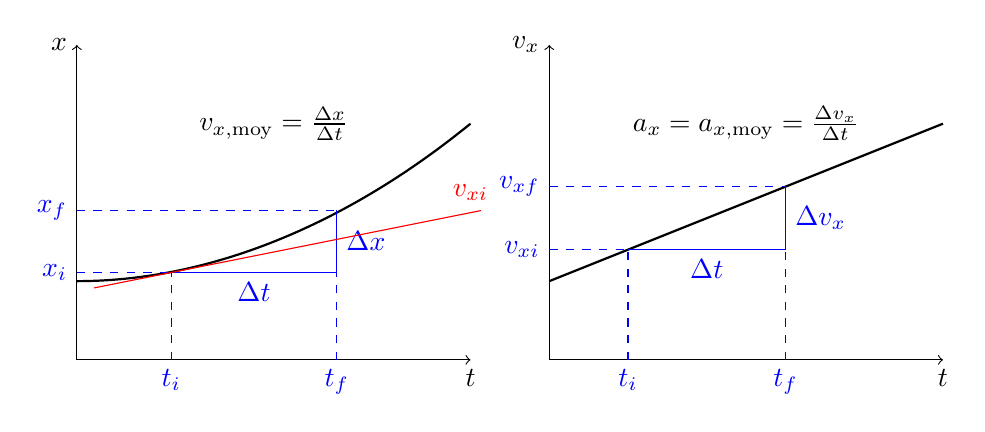
\begin{tikzpicture}
    \draw[->] (0, 0) -- (5, 0) node[below] {$t$};
    \draw[->] (0, 0) -- (0, 4) node[left] {$x$};
    \coordinate (O) at (0, 0);
    \coordinate (A) at (1.2, 1.11);
    \coordinate (B) at (3.3, 1.9);
    \draw[thick] (0, 1) parabola (5, 3);
    \draw[blue] (A) -- node[below] {$\Delta t$} (A -| B)
                -- node[right] {$\Delta x$} (B);
    \draw[dashed, blue] (A |- O) node[below] {$t_i$} -- (A);
    \draw[dashed, blue] (B |- O) node[below] {$t_f$} -- (A -| B);
    \draw[dashed, blue] (O |- A) node[left] {$x_i$} -- (A);
    \draw[dashed, blue] (O |- B) node[left] {$x_f$} -- (B);
    \node at (2.5, 3) {$v_{x, \mathrm{moy}} = \frac{\Delta x}{\Delta t}$};
    \draw[shorten >= -4cm, shorten <= -1cm, red] (A) -- ++(0.01, 0.002);
    \node[red] at (5, 2.13) {$v_{xi}$};
    \begin{scope}[shift={(6, 0)}]
      \draw[->] (0, 0) -- (5, 0) node[below] {$t$};
      \draw[->] (0, 0) -- (0, 4) node[left] {$v_x$};
      \draw[thick] (0, 1) -- (5, 3);
      \draw[blue] (1, 1.4) -- node[below] {$\Delta t$} (3, 1.4)
                  -- node[right] {$\Delta v_x$} (3, 2.2);
      \draw[dashed, blue] (1, 0) node[below] {$t_i$} -- (1, 1.4);
      \draw[dashed, blue] (3, 0) node[below] {$t_f$} -- (3, 1.4);
      \draw[dashed, blue] (0, 1.4) node[left] {$v_{xi}$} -- (1, 1.4);
      \draw[dashed, blue] (0, 2.2) node[left] {$v_{xf}$} -- (3, 2.2);
      \node at (2.5, 3) {$a_x = a_{x, \mathrm{moy}} = \frac{\Delta v_x}{\Delta t}$};
    \end{scope}
  \end{tikzpicture}
  \label{fig:mrua}
  \caption{Position en fonction du temps et vitesse en fonction du temps pour
    un mouvement rectiligne uniformément accéléré.}
\end{figure}
La composante de la vitesse et de l'accélération peuvent être exprimées comme
suit
\begin{align*}
  v_x(t) &= v_{0x} + a_xt \\
  a_x(t) &= a_x
\end{align*}
Pour ce qui est de la position, l'analyse est légèrement plus compliquée et
elle sera faite en détail plus tard dans ce chapitre.


\paragraph{Exemple -- Un mouvement quelconque}

Considérons le mouvement illustré à la figure \ref{fig:quelconque}.

\begin{figure}
  \begin{center}
  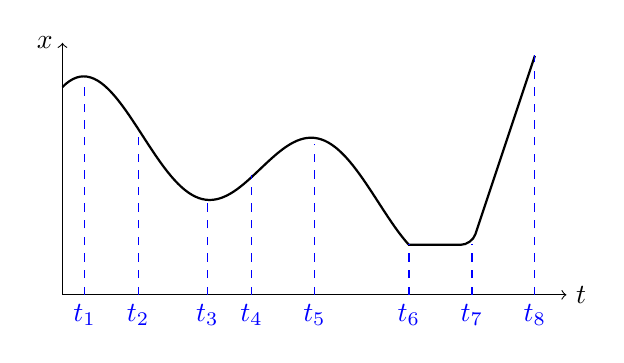
\begin{tikzpicture}[scale=0.8]
    \draw[->] (0, 0) -- (8, 0) node[right] {$t$};
    \draw[->] (0, 0) -- (0, 4) node[left] {$x$};
    \draw[thick] plot[domain=0:5.5, samples=100] (\x, {2 + 1.3*cos(1.5*\x r)+sin(\x r)})
          to[rounded corners] ++(1, 0) -- ++(1, 3);
    \draw[dashed, blue] (0.35, 0) node[below] {$t_1$} -- (0.35, 3.4);
    \draw[dashed, blue] (1.2, 0)  node[below] {$t_2$} -- (1.2, 2.6);
    \draw[dashed, blue] (2.3, 0)  node[below] {$t_3$} -- (2.3, 1.5);
    \draw[dashed, blue] (3, 0)    node[below] {$t_4$} -- (3, 1.9);
    \draw[dashed, blue] (4, 0)    node[below] {$t_5$} -- (4, 2.4);
    \draw[dashed, blue] (5.5, 0)  node[below] {$t_6$} -- (5.5, 0.8);
    \draw[dashed, blue] (6.5, 0)  node[below] {$t_7$} -- (6.5, 0.8);
    \draw[dashed, blue] (7.5, 0)  node[below] {$t_8$} -- (7.5, 3.8);
  \end{tikzpicture}
  \end{center}
  \caption{Position en fonction du temps pour un mouvement quelconque.}
  \label{fig:quelconque}
\end{figure}

Déterminer les intervalles pendant lesquels la vitesse est positive, négative
ou nulle.

Déterminer les intervalles pendant lesquels l'accélération est positive,
négative ou nulle.

La composante de la vitesse est donnée par la pente de la courbe $x$ en
fonction de $t$.  Par conséquent, la vitesse est positive lorsque la pente est
positive, et elle est négative lorsque la pente est négative.

Vitesse positive: $(t_3, t_5)$, $(t_7, t_8)$

Vitesse négative: $(t_1, t_3)$, $(t_5, t_6)$

Vitesse nulle: $t_1$, $t_3$, $t_5$, $(t_6, t_7)$

La composante de l'accélération est positive si la vitesse est en train
d'augmenter, c'est-à-dire si le graphique est courbé vers le haut (comme un
sourire).  L'accélération est négative si le graphique est courbé vers le bas.
Lorsque la courbure du graphique change (on dit qu'il y a un
\textbf{point d'inflexion}), l'accélération est nulle.

Accélération positive: $(t_2, t_4)$

Accélération négative: $[t_1, t_2)$, $(t_4, t_6]$

Accélération nulle: $t_2$, $t_4$, $(t_6, t_7)$, $(t_7, t_8]$


\paragraph{Exemple -- Calculs numériques I}
Considérons le mouvement illustré à la figure suivante.

\begin{center}
\begin{tikzpicture}[scale=0.7]
  \draw[->] (0, 0) -- (8, 0) node[right] {$t (\si{\second})$};
  \draw[->] (0, 0) -- (0, 4) node[left] {$x (\si{m})$};
  \coordinate (O) at (0, 0);
  \coordinate (A) at (1, 3);
  \coordinate (B) at (3, 1);
  \coordinate (C) at (4, 1);
  \coordinate (D) at (5, 3);
  \draw[thick] (O |- A) node[left] {$3$} -- (A) -- (B) -- (C) -- (D) -- ++(2, 0);
  \draw[dashed, blue] (O -| A)  node[below, black] {\num{1}} -- (A);
  \draw[dashed, blue] (O -| B)  node[below, black] {\num{3}} -- (B);
  \draw[dashed, blue] (O -| C)  node[below, black] {\num{4}} -- (C);
  \draw[dashed, blue] (O -| D)  node[below, black] {\num{5}} -- (D);
  \draw[dashed, blue] (O |- B)  node[left, black]  {\num{1}} -- (B);
  \foreach \x in {0,1,...,7} {
    \draw (\x, 0) -- (\x, -0.1);
  }
  \foreach \y in {0,1,...,3} {
    \draw (0, \y) -- (-0.1, \y);
  }
\end{tikzpicture}
\end{center}

Calculer les quantités suivantes:

\begin{tabular}{ll}
  la vitesse moyenne entre \SI{1,2}{\second} et \SI{2}{\second}.
  & \color{blue}{$v_{\mathrm{moy},x} = \SI{-1.00}{\meter\per\second}$} \\
  
  la vitesse instantanée à \SI{4.7}{\second}.
  & \color{blue}{$v_x = \SI{2.00}{\meter\per\second}$} \\

  la distance parcourue entre \SI{0}{\second} et \SI{6}{\second}.
  & \color{blue}{$d = \SI{4.00}{\meter}$} \\

  la vitesse scalaire moyenne entre \SI{0}{\second} et \SI{6}{\second}.
  & \color{blue}{$v_s = \SI{0.667}{\meter\per\second}$} \\

  le déplacement entre \SI{0}{\second} et \SI{4.5}{\second}.
  & \color{blue}{$\Delta x = \SI{-1.00}{\meter}$} \\

  l'accélération moyenne entre \SI{2.5}{\second} et \SI{3.5}{\second}.
  & \color{blue}{$a_{\mathrm{moy}, x} = \SI{1.00}{\meter\per\second\squared}$} \\
\end{tabular}


\paragraph{Exemple -- Calculs numériques II}
Considérons le mouvement illustré à la figure suivante.

\begin{center}
\begin{tikzpicture}[scale=0.7]
  \draw[->] (0, 0) -- (8, 0) node[right] {$t (\si{\second})$};
  \draw[->] (0, -2) -- (0, 4) node[left] {$v_x (\si{m\per\second})$};
  \coordinate (O) at (0, 0);
  \coordinate (A) at (1, 3);
  \coordinate (B) at (3, -1);
  \coordinate (C) at (4, -1);
  \coordinate (D) at (5, 3);
  \draw[thick] (O |- A) node[left] {$3$} -- (A) -- (B) -- (C) -- (D) -- ++(2, 0);
  \draw[dashed, blue] (O -| A)  node[below, black] {\num{1}} -- (A);
  \draw[dashed, blue] (O -| B)  node[above, black] {\num{3}} -- (B);
  \draw[dashed, blue] (O -| C)  node[above, black] {\num{4}} -- (C);
  \draw[dashed, blue] (O -| D)  node[below, black] {\num{5}} -- (D);
  \draw[dashed, blue] (O |- B)  node[left, black]  {\num{-1}} -- (B);
  \foreach \x in {0,1,...,7} {
    \draw (\x, 0) -- (\x, -0.1);
  }
  \foreach \y in {-2,-1,...,3} {
    \draw (0, \y) -- (-0.1, \y);
  }
\end{tikzpicture}
\end{center}

Calculer les quantités suivantes:

\begin{tabular}{ll}
  la vitesse instantanée à \SI{2}{\second}.
  & \color{blue}{$v_{x} = \SI{1.00}{\meter\per\second}$} \\
  
  l'accélération moyenne entre \SI{3}{\second} et \SI{6}{\second}.
  & \color{blue}{$a_{\mathrm{moy},x} = \SI{1.33}{\meter\per\second\squared}$} \\

  l'accélération instantanée à \SI{3.5}{\second}.
  & \color{blue}{$a_x = \SI{0.00}{\meter\per\second\squared}$} \\

  le déplacement entre \SI{3}{\second} et \SI{4}{\second}.
  & \color{blue}{$\Delta x = \SI{-1.00}{\meter}$} \\

  les temps auxquels la direction change.
  & \color{blue}{$\SI{2.50}{\second}$ et \SI{4.25}{\second}} \\

  les temps auxquels l'objet est immobile.
  & \color{blue}{$\SI{2.50}{\second}$ et \SI{4.25}{\second}} \\
\end{tabular}


\subsection{Aires, déplacements et vitesses}

On a vu que la vitesse est la pente du graphe de la position en fonction du
temps et l'accélération est la pente du graphe de la vitesse en fonction du
\marginnote{
\[
  x \xrightarrow{\mathrm{pente}\, \left(\der{}{x}\right)} v_x
  \xrightarrow{\mathrm{pente}\, \left(\der{}{x}\right)} a_x
\]
}
temps.  Ces relations sont résumées dans le schéma à ci-contre.

Il existe également des relations qui nous permettent de déterminer la position
et la vitesse à partir des graphiques de la vitesse et de l'accélération en
fonction du temps.  Ces relations nous permettront de déterminer l'équation qui
décrit la position en fonction du temps pour un mouvement rectiligne
uniformément accéléré.

Considérons d'abord un mouvement rectiligne uniforme.  L'accélération est nulle
et la vitesse est constante.  Le graphique de la vitesse en fonction du temps
est donc une droite horizontale.  Supposons qu'une balle de tennis est servie à
une vitesse de module \SI{200}{\kilo\meter\per\hour}.  \marginnote{Le service
  le plus rapide jamais enregistré était celui de Samuel Groth, un joueur
  australien.  Ce service a eu lieu au \textit{ATP Challenger} à Busan, en
  Corée du Sud, en mai 2012 et avait une vitesse de module
  \SI{263}{\kilo\meter\per\hour}}
La distance parcourue par cette balle en une seconde est
\begin{align*}
  d &= v \Delta t \\
    &= \SI{200}{\kilo\meter\per\hour} \times \SI{1}{\second} \\
    &= \SI{200}{\kilo\meter\per\hour} \times \SI{1}{\second}
       \times \frac{\SI{1}{\hour}}{\SI{3600}{\second}}
       \times \frac{\SI{1000}{\meter}}{\SI{1}{\kilo\meter}} \\
    &= \SI{55.6}{\meter}
\end{align*}
En général, pour connaître le déplacement effectué
entre deux instants $t_i$ et $t_f$, on peut tout simplement multiplier la
composante de la vitesse par l'intervalle de temps:
\[
  \Delta x = v_x \Delta t = v_x (t_f - t_i)
\]
Graphiquement, ce calcul est équivalent à trouver l'aire de la région comprise
entre le graphique de $v$ et fonction du temps et l'axe des abscisses.

\begin{marginfigure}
    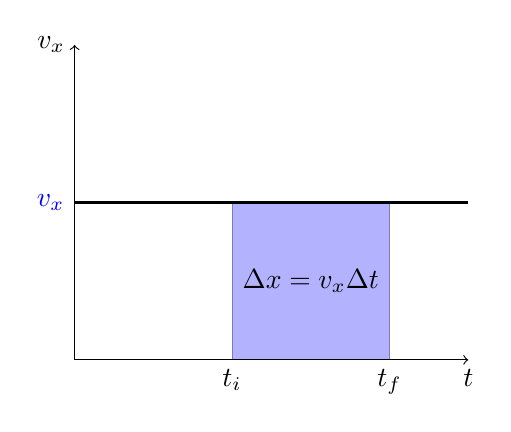
\begin{tikzpicture}
      \draw[fill=blue, opacity=0.3] (2, 0) rectangle (4, 2);
      \draw[->] (0, 0) -- (5, 0) node[below] {$t$};
      \draw[->] (0, 0) -- (0, 4) node[left] {$v_x$};
      \draw[thick] (0, 2) node[left, blue] {$v_x$} -- (5, 2);
      \node[below] at (2, 0) {$t_i$};
      \node[below] at (4, 0) {$t_f$};
      \node at (3, 1) {$\Delta x = v_x \Delta t$};
  \end{tikzpicture}
  \label{fig:mru_vx}
  \caption{Vitesse en fonction du temps pour
    un mouvement rectiligne uniforme.}
\end{marginfigure}

En remarquant que $\Delta x = x_f - x_0$ et en posant que $t_i = 0$, on obtient
l'équation
\[
  x_f = x_0 + v_xt_f
\]
qu'on réécrit souvent en laissant tomber les indices $f$ pour obtenir
l'équation linéaire dont nous avons parlé précédemment
\[
  x(t) = x_0 + v_x t
\]

Pour que l'interprétation des aires comme des déplacements soit correcte, il
faut que l'on puisse tenir compte du fait qu'un déplacement peut aussi avoir
une composante négative.  Si on considère les aires sous l'axe des abscisses
comme négatives, alors les ``aires'' et les déplacements seront les mêmes.

Dans un mouvement rectiligne uniformément accéléré, l'accélération est
constante et la vitesse varie de façon linéaire.  Le graphique de la vitesse en
fonction du temps est illustré à la figure \ref{fig:mrua_aire}.  On peut
considérer le mouvement comme étant composé de plusieurs mouvements à vitesse
constante, l'un à la suite de l'autre, avec la vitesse qui augment entre chacun
de ces petits sous-mouvements.  On constate alors que l'aire sous la courbe
donne encore une fois le déplacement.  Cette fois, l'aire peut être calculée à
partir de la formule de l'aire d'un trapèze, ou simplement en divisant le
trapèze en un rectangle et un triangle.

\begin{marginfigure}
  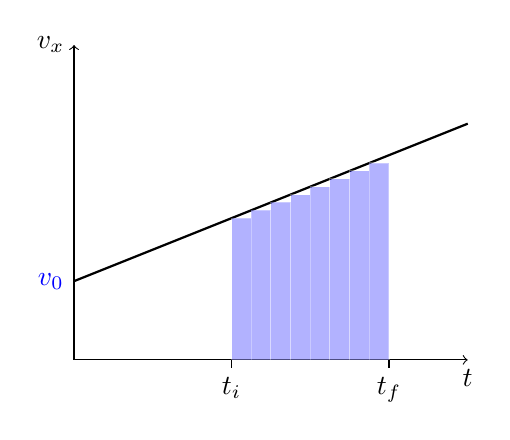
\begin{tikzpicture}[scale=1]
      \draw[->] (0, 0) -- (5, 0) node[below] {$t$};
      \draw[->] (0, 0) -- (0, 4) node[left] {$v_x$};
      \draw[thick] (0, 1) node[left, blue] {$v_0$} -- (5, 3);
      \foreach \x in {0, 0.25, ..., 1.75} {
        \draw[white, fill=blue, opacity=0.3] (2 + \x, 0)
             rectangle (2 + \x + 0.25, 1.8 + \x*0.4);
      }
      \draw (2, 0) -- ++(0, -0.1) node[below] {$t_i$};
      \draw (4, 0) -- ++(0, -0.1) node[below] {$t_f$};
  \end{tikzpicture}
  \caption{Mouvement rectiligne uniformément accéléré}
  \label{fig:mrua_aire}
\end{marginfigure}

L'aire du rectangle est $v_i\Delta t$ alors que l'aire du triangle est
$\frac{1}{2}(v_f - v_i)\Delta t$.  En combinant ces deux expressions on arrive
à
\[
  \Delta x = v_i \Delta t + \frac{1}{2} (v_f - v_i) \Delta t
\]
Encore une fois, on peut considérer $t_i = 0$ et laisser tomber les indices
$f$.  Alors l'équation devient
\begin{align*}
  x - x_0 &= v_{0x} t + \frac{1}{2} (v_x - v_{0x}) t
\end{align*}
Comme on considère un mouvement uniformément accéléré, on peut écrire la
vitesse comme $v_x(t) = v_0 + a_x t$.  En substituant dans l'équation
précédente et en simplifiant on obtient
\[
  x(t) = x_0 + v_{0x} t + \frac{1}{2} a_x t^2
\]

\marginnote{
\[
  x \xrightleftharpoons[\mathrm{aire}\, \left(\int \dif x\right)]{\mathrm{pente}\, \left(\der{}{x}\right)} v_x
  \xrightleftharpoons[\mathrm{aire}\, \left(\int \dif x\right)]{\mathrm{pente}\, \left(\der{}{x}\right)} a_x
\]
}
En résumé, l'aire entre la courbe de la vitesse en fonction du temps et l'axe
des abscisses donne le déplacement.  De même, l'aire entre la courbe de
l'accélération en fonction du temps et l'axe des abscisses donne la vitesse.
On peut ainsi compléter notre diagramme qui relie position, vitesse et
accélération.  Le calcul d'aires sous un graphique correspond à calculer une
intégrale.


\subsection{Les équations de la cinématique à une dimension}

Dans les sections précédentes, nous avons appris des méthodes générales pour
relier la position, la vitesse et l'accélération.  En cours de route, nous
avons déterminer toutes les équations de la cinématique pour le mouvement
rectiligne uniforme et pour le mouvement rectiligne uniformément accéléré.  Ces
équations sont résumées ici.

\begin{tabular}{lll}
  \toprule
               & MRU   & MRUA \\
  \midrule
  Position     & $x(t) = x_0 + v_xt$  &  $x(t) = x_0 + v_{0x}t + \frac{1}{2}a_x t^2$ \\
  Vitesse      & $v_x(t) = v_0x$       &  $v_x(t) = v_{0x} + a_x t$    \\
  Accélération & $a_x(t) = 0$         &  $a_x(t) = a_{0x}$    \\
  \bottomrule
\end{tabular}

\subsection{Exercice -- MRUA I -- Freinage en voiture}

Un conducteur dans sa voiture voit un piéton à \SI{30}{\meter} devant lui.  À
ce moment, il décide d'appliquer les freins pour tenter d'éviter de frapper le
piéton.  À partir du moment où il appuie sur la pédale de frein, on suppose que
son accélération a un module constant.  Il parvient à arrêter sa voiture juste
avant d'atteindre le piéton.

\begin{marginfigure}
  \includegraphics[scale=0.3]{03_Cinematique/2014porsche911gt3.jpg}
  \caption{Une Porsche 911 GT3 2014 peut freiner avec une accélération de
    module \SI{11.9}{\meter\per\second\squared}.}
  \label{fig:porsche}
\end{marginfigure}

En général, entre le moment où un conducteur décide de freiner et le moment où
il commence à appuyer sur la pédale de frein, il s'écoule \SI{1.3}{\second}.
On suppose que notre conducteur est un pilote professionnel et que son temps de
réaction est plutôt \SI{1}{s}.

\begin{marginfigure}
  \includegraphics[scale=0.3]{03_Cinematique/2012toyota_yaris.jpg}
  \caption{Une Toyota Yaris 2012 peut freiner avec une accélération de
    module \SI{9.29}{\meter\per\second\squared}.  Les modèles plus lourds,
    comme la Prius V 2013 n'atteignent que des accélérations de module
    \SI{8.41}{\meter\per\second\squared}.}
  \label{fig:porsche}
\end{marginfigure}

La majorité des voitures ont un module d'accélération maximal lors
d'un freinage situé entre \SI{7.5}{\meter\per\second\squared} et
\SI{9.8}{\meter\per\second\squared}.  On suppose que notre conducteur possède
une excellente voiture sport munie de pneus neufs et d'excellente qualité.
Grâce à cela, il peut freiner avec une accélération de module
\SI{11.9}{\meter\per\second\squared}.

\marginnote{\vspace{0.2cm}

  Les données sur les accélérations et les images proviennent du site
  \url{http://www.caranddriver.com/list-reviews-instrumented-tests/}. Le site
  contient une description détaillée du protocole expérimental utilisé pour
  faire les mesures de freinage.

  Le temps de réaction pour le freinage provient du dépliant \emph{Sur la
  route, prenez le temps de ralentir} publié par la SAAQ et disponible à
  l'adresse
  \url{http://www.saaq.gouv.qc.ca/publications/prevention/route_ralentir.pdf}.

  L'impact d'une chaussée mouillé a été déterminé à partir des données fournies
  par la police fédérale australienne
  \url{http://www.police.act.gov.au/roads-and-traffic/speeding/stopping-distances-explained.aspx}.
}

\begin{enumerate}[a]
  \item Déterminer la vitesse à laquelle la voiture se déplaçait
    lorsque le conducteur a aperçu le piéton.
  \item Sur une chaussée mouillée, le module maximal de l'accélération est
    réduit de \SI{35}{\percent}.  Si la voiture se déplaçait à la vitesse
    calculée en (a), à quelle vitesse aurait-elle percuté le piéton sur une
    chaussée mouillée?
  \item Supposons à nouveau que la chaussée est sèche.  Si le conducteur allait
    \SI{5}{\kilo\meter\per\hour} plus vite que la vitesse calculée en (a), à
    quelle vitesse aurait-il percuté le piéton?
\end{enumerate}

\paragraph{Solution}

\begin{enumerate}[a]
  \begin{marginfigure}
    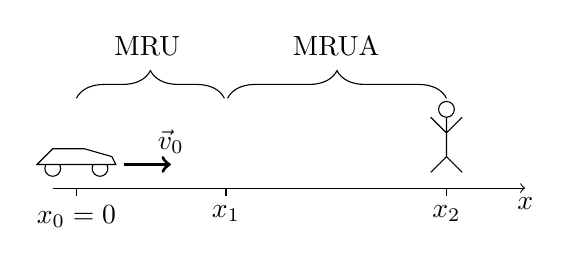
\begin{tikzpicture}[scale=1]
      \draw[->] (0, 0) -- (6, 0) node[below] {$x$};
      \draw (0.3, 0) -- (0.3, -0.1) node[below] {$x_0 = 0$};
      \draw (2.2, 0) -- (2.2, -0.1) node[below] {$x_1$};
      \draw (5, 0) -- (5, -0.1) node[below] {$x_2$};
      \draw (5, 1) circle (0.1);
      \draw (5, 0.9) -- (5, 0.4) -- (4.8, 0.2)
            (5, 0.4) -- (5.2, 0.2)
            (5, 0.7) -- (4.8, 0.9)
            (5, 0.7) -- (5.2, 0.9);
    \draw (0.6, 0.25) circle (0.1);
    \draw (0, 0.25) circle (0.1);
    \draw[fill=white] (-0.2, 0.3) -- (0.8, 0.3) -- (0.75, 0.4) -- (0.4, 0.5) -- (0, 0.5) -- cycle;
    \draw[->, very thick] (0.9, 0.3) -- (1.5, 0.3) node[above] {$\vec{v}_0$};
    \draw [decorate,decoration={brace,amplitude=10pt,raise=4pt},yshift=0pt] (0.3, 1) -- (2.18, 1);
    \node at (1.2, 1.8) {MRU};
    \draw [decorate,decoration={brace,amplitude=10pt,raise=4pt},yshift=0pt] (2.22, 1) -- (5, 1);
    \node at (3.6, 1.8) {MRUA};
    \end{tikzpicture}
  \end{marginfigure}
  \item On décompose le temps d'arrêt en deux parties: le temps entre le moment
    où le conducteur voit le piéton ($t_0 = \SI{0}{\second}$) et celui où il
    appuie sur le frein ($t_1$), et le temps entre le moment où il appuie sur
    le frein et celui où la voiture arrête ($t_2$).  Entre $t_0$ et $t_1$, la
    voiture avance à vitesse constante et donc son mouvement est rectiligne
    uniforme.  Entre $t_1$ et $t_2$, le conducteur freine et la voiture est
    donc en mouvement rectiligne uniformément accéléré.

    Soit $x_0$, $x_1$ et $x_2$ les positions aux temps $t_0$, $t_1$ et $t_2$
    respectivement; soit $v_0$ le module de la vitesse initiale.  

    On cherche $v_{0}$.

    On connaît les quantités suivantes:
    \begin{enumerate}[i.]
      \item $v_{2x} = \SI{0}{\meter\per\second}$
      \item $x_0 = \SI{0}{\meter}$
      \item $x_2 = \SI{30}{\meter}$
      \item $t_0 = \SI{0}{\second}$
      \item $t_1 = \SI{1}{\second}$
    \end{enumerate}

    \begin{marginfigure}
    \begin{tikzpicture}[scale=1]
      \draw[->] (0, 0) -- (6, 0) node[below] {$t$};
      \draw[->] (0, 0) -- (0, 5) node[left] {$v_{x}$};
      \draw[thick] (0, 3) node[left] {$v_{0x}$} -- (2, 3) -- (5, 0);
      \draw[dashed] (2, 3) -- (2, 0) node[below] {$t_1$};
      \node[below] at (5, 0) {$t_2$};
    \end{tikzpicture}
    \end{marginfigure}

    La position finale de la voiture est la même que la position du piéton.
    Puisque la position initiale est \SI{0}{\meter}, le déplacement lors du MRU
    plus le déplacement lors du MRUA doit être égal à $x_2$:
    \[
      x_2 = \Delta x_\mathrm{MRU} + \Delta x_\mathrm{MRUA}
    \]
    Pour le MRU, l'intervalle de temps est entre $0$ et $t_1$ donc
    \begin{align*}
      \Delta x_\mathrm{MRU} = v_{0x} t_1
    \end{align*}
    Pour le MRUA, l'intervalle de temps est entre $t_1$ et $t_2$.
    \begin{align*}
      \Delta x_\mathrm{MRUA} = v_{0x} (t_2 - t_1) + \frac{1}{2} a_x (t_2 -
                               t_1)^2
    \end{align*}
    En combinant les deux on obtient
    \begin{align}
      x_2 &= v_{0x} t_1 + v_{0x} (t_2 - t_1) + \frac{1}{2} a_x (t_2 -
                               t_1)^2 \label{eqn:car1}
    \end{align}
    On a une équation avec deux inconnues $v_{0x}$ et $t_2$.  Il nous faut une
    autre équation pour résoudre le problème.  La seule information que nous
    n'avons toujours par utilisée est le fait que la vitesse finale est nulle.
    On sait que la deuxième partie du mouvement est un MRUA donc
    \begin{equation}
      v_{2x} = v_{0x} + a_x (t_2 - t_1)
      \label{eqn:car2}
    \end{equation}
    et cette expression se simplifie parce que $v_{2x} =
    \SI{0}{\meter\per\second}$:
    \begin{equation}
      \SI{0}{\meter\per\second} = v_{0x} + a_x (t_2 - t_1)
      \label{eqn:car3}
    \end{equation}
    On peut isoler $t_2 - t_1$ dans l'équation \ref{eqn:car3} et substituer dans
    l'équation \ref{eqn:car1}.
    \begin{align*}
      t_2 - t_1 &= \frac{- v_{0x}}{a_x} \\
      x_2 &= v_{0x} t_1 + v_{0x} \frac{- v_{0x}}{a_x} + \frac{1}{2} a_x
             \left(\frac{- v_{0x}}{a_x}\right)^2 \\
          &= v_{0x} t_1 - \frac{1}{2} \frac{v_{0x}^2}{a_x}
    \end{align*}
    Cette équation est quadratique en $v_{0x}$.  On peut donc la résoudre avec
    la formule quadratique.  Tout d'abord on la récrit dans la forme habituelle 
    \[
      \frac{1}{2a_x} v_{0x}^2 - t_1v_{0x} + x_2 = 0
    \]
    puis on applique la formule
    \begin{align*}
      v_{0x} &= \frac{t_1 \pm \sqrt{t_1^2 - 4x_2 / (2a_x)}}{1/a_x} \\
             &= a_x\left( t_1 \pm \sqrt{t_1^2 - 2x_2 / a_x} \right)
    \end{align*}
    On sait que la composante de la vitesse est positive alors que la
    composante de l'accélération est négative, par conséquent, seule la
    solution avec le ``$-$'' est physiquement possible.
    \begin{align*}
      v_{0x} &= a_x\left( t_1 - \sqrt{t_1^2 - 2x_2 / a_x} \right) \\
             &= \SI{17.3508}{\meter\per\second} \\
             &= \SI{62.4629}{\kilo\meter\per\hour}
    \end{align*}
    \[
      \boxed{v_{0x} = \SI{17.4}{\meter\per\second}}
    \]


  \item Si la chaussée est mouillée, le module de l'accélération diminue de
    \SI{35}{\percent}, donc
    \[
      a_{mx} = \num{0.65} a_x = -\SI{7.735}{\meter\per\second\squared}
    \]
    On connaît la vitesse initiale
    \[
      v_{0x} = \SI{17.3508}{\meter\per\second}
    \]
    et on cherche la vitesse finale, c'est-à-dire lorsque la voiture atteint le
    piéton.

    Pendant le MRU, la voiture fait un déplacement
    \begin{align*}
      \Delta x_\mathrm{MRU} = v_{0x} t_{1}.
    \end{align*}
    Lorsque le chauffeur commence à appuyer sur les freins, il est donc à la
    position $x_i = v_{0x} t_{1}$.

    Lors du MRUA, la vitesse en fonction du temps est donnée par
    \[
      v_x = v_{0x} + a_{mx} t'
    \]
    où $t'$ est le temps depuis le début du MRUA (donc $t' = t - t_1$).  Si on
    élève cette expression au carré, on obtient
    \begin{align*}
      v_x^2 &= \left( v_{0x} + a_{mx} t' \right)^2 \\
            &= v_{0x}^2 + 2v_{0x} a_{mx} t' + a_x^2 t'^2 \\
            &= v_{0x}^2 + 2a_{mx}\left(v_{0x} t' + \frac{1}{2} a_{mx} t'^2\right) \\
      v_x^2 &= v_{0x}^2 + 2a_{mx}\left( x - x_i \right) \\
    \end{align*}
    Si on applique cette relation à l'instant où la voiture frappe le piéton,
    $x = \SI{30}{\meter}$ et $v_{x}$ est la vitesse recherchée.
    \begin{align*}
      v_x &= \sqrt{v_{0x}^2 + 2a_{mx}\left( x - x_i \right)} \\
          &= \sqrt{v_{0x}^2 + 2a_{mx}\left( x - v_{0x}t_1 \right)} \\
          &= \SI{10.2648}{\meter\per\second} \\
          &= \SI{36.9534}{\kilo\meter\per\second}
    \end{align*}
    \[
      \boxed{v_x = \SI{10.3}{\meter\per\second}}
    \]


  \item Ici, la vitesse initiale est
    \begin{align*}
      v_{0x} &= \SI{62.4629}{\kilo\meter\per\hour} +
                \SI{5}{\kilo\meter\per\hour} \\
             &= \SI{18.7397}{\meter\per\second}
    \end{align*}
    On peut appliquer exactement la même formule qu'à la question précédente.
    \begin{align*}
      v_x &= \sqrt{v_{0x}^2 + 2a_{x}\left( x - v_{0x}t_1 \right)} \\
          &= \SI{9.12037}{\meter\per\second} \\
          &= \SI{32.8333}{\kilo\meter\per\second}
    \end{align*}
    \[
      \boxed{v_x = \SI{9.12}{\meter\per\second}}
    \]



\end{enumerate}


\subsection{Exercice -- MRUA II -- Partie de football}

Un joueur de football des Alouettes court vers la zone de touche de l'équipe
adverse, les Stampeders, à une vitesse constante de \SI{10}{\meter\per\second}.
Lorsqu'il franchit la ligne de $40$ verges de son côté du terrain, un
coéquipier lui passe le ballon.  \SI{0.8}{\second} après que le joueur des
Alouettes ait reçu le ballon, un joueur des Stampeders situé en face, à la
ligne de $20$ verges du côté des Stampeders, se lance vers lui à partir du
repos.  On suppose que le joueur des Stampeders a une accélération constante.

\begin{marginfigure}
  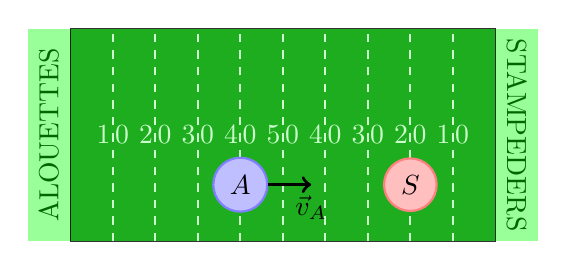
\begin{tikzpicture}[scale=0.9]
    \fill[green!40] (-0.6, 0) rectangle (6.6, 3);
    \draw[opacity=0.8, fill=green!60!black] (0, 0) rectangle (6, 3);
    \draw[thick, green!20!white, dashed] (3, 0) -- node {$5\,0$} (3, 3);
    \foreach \i in {1, 2, ..., 4} {
      \draw[thick, green!20!white, dashed] (0.6*\i, 0) -- node {$\i\,0$} (0.6*\i, 3);
      \draw[thick, green!20!white, dashed] (6-0.6*\i, 0) -- node {$\i\,0$} (6-0.6*\i, 3);
    }
    \node[rotate=90, green!40!black] at (-0.3, 1.5) {ALOUETTES};
    \node[rotate=-90, green!40!black] at (6.3, 1.5) {STAMPEDERS};
    \node[circle, fill=blue!25, thick, draw=blue!50!white] (A) at (2.4, 0.8) {$A$};
    \node[circle, fill=red!25, thick, draw=red!50!white] at (4.8, 0.8) {$S$};
    \draw[very thick, ->] (A) -- ++(1, 0) node[below] {$\vec{v}_{A}$};
  \end{tikzpicture}
  \caption{Position des deux joueurs au moment où le joueur des Alouettes
    reçoit le ballon.  Le joueur des Alouettes est représenté par un $A$ et
    celui des Stampeders par un $S$.}
  \label{fig:football}
\end{marginfigure}

Si les deux joueurs entrent en collision \SI{2}{\second} après le départ du
joueur des Stampeders déterminer les quantités suivantes:

\begin{enumerate}
  \item l'accélération du joueur des Stampeders;
  \item la vitesse du joueur des Stampeders lors de la collision;
  \item la position des joueurs lors de la collision;
\end{enumerate}

\textit{Note: Une verge est égale à \SI{0.9144}{\meter}.}

\paragraph{Solution}

Posons que le temps auquel le joueur $A$ reçoit le ballon est $t =
\SI{0}{\second}$.  Le joueur $A$ est toujours en mouvement rectiligne uniforme
alors que je joueur $S$ est au repos pendant \SI{0.8}{\second} puis il est en
mouvement rectiligne uniformément accéléré pour la suite.  On pose aussi que la
position initiale de $A$ est à $x = \SI{0}{\meter}$.

Soit $x_A$ la position de $A$. On sait que
\[
  x_A(t) = v_{Ax} t.
\]
Dans le cas de $S$, sa position ne commence à changer qu'à partir de $t =
\SI{0.8}{\second}$.  Sa position initiale est $x_{S0} = 40\, \mathrm{verges}$.
Une fois qu'il a commencé à courir, sa position est donnée par un MRUA, mais il
faut tenir compte du fait que le temps pendant lequel il a couru est en réalité
$t - \SI{0.8}{\second}$:
\[
  x_S(t) = x_{S0} + v_{S0} (t - \SI{0.8}{\second})
           + \frac{1}{2} a_x (t - \SI{0.8}{\second})^2
\]
Puisqu'il part du repos, sa vitesse initiale est nulle et donc
\[
  x_S(t) =  x_{S0} + \frac{1}{2} a_x (t - \SI{0.8}{\second})^2
\]

La collision a lieu lorsque la position des deux joueurs est la même, i.e.:
\begin{align*}
  x_A &= x_S \\
  v_{Ax} t_\mathrm{collision} &= x_{S0} + \frac{1}{2} a_x (t_\mathrm{collision} - \SI{0.8}{\second})^2
\end{align*}
et on sait que la collision a lieu à $t_\mathrm{collision} = \SI{2.8}{s}$.
L'équation précédente ne contient qu'une seule inconnue, soit l'accélération.
Un peu d'algèbre donne
\[
  a_x = \frac{2\left(v_{Ax} t_\mathrm{collision} - x_{S0}\right)}
             {(t_\mathrm{collision} - \SI{0.8}{\second})^2}
\]
\[
  \boxed{a_x = \SI{-4.29}{\meter\per\second\squared}}
\]

Une fois qu'on connaît l'accélération, il est facile de déterminer la vitesse
du joueur des Stampeders:
\begin{align*}
  v_{Sfx} = a_x (t_\mathrm{collision} - \SI{0.8}{\second})
\end{align*}
\[
  \boxed{v_{Sfx} = \SI{-8.58}{\meter\per\second}}
\]

On peut calculer la position de la collision simplement à partir de la vitesse
du joueur $A$ et du temps avant que la collision ne se produise.
\begin{align*}
  x_\mathrm{collision} &= v_{Ax} t_\mathrm{collision}
\end{align*}
\[
  \boxed{x_\mathrm{collision} = \SI{28.0}{\meter} = \num{30.6}\,\mathrm{verges}}
\]
Autrement dit, le joueur des Alouettes aura tout juste le temps de franchir la
ligne de \num{30} verges du côté des Stampeders avant d'être plaqué.


